\documentclass[a4paper]{article}
\usepackage[margin=1in]{geometry}
\usepackage{titlesec}
\usepackage{xcolor}
\usepackage[colorlinks=true,linkcolor=blue,urlcolor=blue,citecolor=blue]{hyperref}
\usepackage{listings}
\usepackage{graphicx}
\usepackage{float}
\usepackage{booktabs}
\usepackage{enumitem}
\usepackage{fancyhdr}
\usepackage{verbatim}
\usepackage{tikz}
\usepackage{svg}
\usetikzlibrary{shapes.geometric, arrows.meta, positioning, fit, backgrounds}

% Define a dark-accented color for section rule lines
\definecolor{DarkAccent}{HTML}{1F2937}

% Set up titlesec styling
\titleformat{\section}
  {\normalfont\Large\bfseries\color{DarkAccent}}{\thesection.}{0.5em}{}[{\titlerule[0.8pt]}]

% Page layout setup with fancyhdr
\pagestyle{fancy}
\fancyhf{}
\fancyhead[L]{Interactive Multi-Core CPU Scheduling Simulator}
\fancyfoot[C]{\thepage}
\renewcommand{\headrulewidth}{0.4pt}

\begin{document}

\title{\vspace{-2cm}Interactive Multi-Core CPU Scheduling Simulator \\
\large An Educational OS Scheduling Visualization Platform}
\author{Syed Arsh Ahmad \and Kanwar Aaryaman Singh \and Ayan Kar}
\date{\today}

\maketitle

\section*{Abstract}
The project aims to build an educational data-visualization web application mapping Operating System process scheduling inside modern multi-core processors. It serves as an interactive platform designed to bridge theoretical concepts and real-world execution. By modeling highly concurrent processing load distributions, the application visualizes the systemic logic behind algorithms such as First Come First Serve, Work Stealing, and CPU Affinity directly within the browser, providing a sandbox for dynamically spanning CPU bursts and analyzing core utilization.

\section{Project Overview}
The Interactive Multi-Core CPU Scheduling Simulator is a high-performance, dynamic application intended to visually demonstrate how operating systems handle process distribution tasks across multiple processing units. Designed as an educational sandbox, its purpose separates algorithmic theory from textbooks and renders it into a realistic layout tracking global queues, historical metrics, and thread execution states, empowering users to dynamically switch logic pathways on the fly. 

\section{Module-Wise Breakdown}

\subsection{Simulation Engine \& State Controller}
The backbone of the application. It acts as the primary system clock, advancing the simulation continuously while maintaining the state of the global queue and individual core assignments. It is heavily decoupled into a set of custom React Hooks (primarily \texttt{useSimulation}), which strictly isolate the complex mathematical evaluation arrays from the rendering logic. This module manages complete process life-cycles, enforces strict algorithmic rules, calculates dynamic time quantums explicitly, and manages the intricate context-switching mechanics necessary for accurate metric tracking execution.

\subsection{Interactive GUI \& Process Visualizer}
The front-end user interface responsible for dynamically rendering the underlying system state. This module orchestrates the visual representation of active CPU cores, pending queues, and historical execution timelines using extremely fast layout transitions. By leveraging modern DOM rendering through React 19 and Framer Motion, it effectively translates flat arrays of backend objects into smooth, tangible floating components without noticeable layout shifts, providing constant interactive feedback through tooltips, fluid hover mechanics, and robust, context-aware variable color-coded status mappings.

\subsection{Analytics \& Benchmarking}
A dedicated subsystem tracking historical execution metrics. It captures complex metrics such as theoretical throughput, average response times, aggregated process wait times, task migration counts, and CPU utilization balance across the multi-core environment, presenting them natively as responsive interactive charts. This module seamlessly aggregates data on every precise internal ticking cycle without inducing computational freezes, feeding parsed datasets directly to SVG-based Recharts rendering blocks perfectly mapped against axis constraints.

\section{Functionalities}

\subsection{Simulation Engine \& State Controller}
\begin{itemize}[noitemsep]
    \item \textbf{Dynamic Scheduling Capabilities:} Capable of seamlessly running 8 distinct, algorithmically complex paths including Round Robin, Shortest Job First, Work Stealing, Push/Pull Migration, Completely Fair Scheduler, and strict CPU Affinity configurations. Users can hot-swap these algorithms efficiently at runtime without forcing memory resets.
    \item \textbf{Auto-Spawning Mechanics:} Procedurally generates mathematically realistic user workloads continuously throughout execution cycles, modeling real-world chaotic software burst demands safely.
    \item \textbf{Load Balancing Logic:} Employs aggressive heuristic arrays to effectively balance continuous processor workloads, actively avoiding pipeline bottlenecks by transferring execution queues completely away from locked or overloaded internal logic kernels.
\end{itemize}

\subsection{Interactive GUI \& Process Visualizer}
\begin{itemize}[noitemsep]
    \item \textbf{Per-Core Dashboards:} Live, pinpoint rendering of individual mapped CPU utilization percentages, currently active locked running processes, and granularly nested core-dependent operational queues equipped securely with responsive completion progress tracking bars.
    \item \textbf{Gantt Chart Timeline:} An animated, chronologically scrollable execution timeline continuously tracking complete processes. It actively offers clear tooltip clarity explicitly detailing isolated context bounds routed directly to historic core allocation pathways securely.
    \item \textbf{Custom Parameter Entry:} Allows proactive analytical users unparalleled layout access to manually inject precise functional tasks equipped exclusively with discrete execution constraints, prioritized overrides, and independent scaling masking limits.
\end{itemize}

\subsection{Analytics \& Benchmarking}
\begin{itemize}[noitemsep]
    \item \textbf{Live Metric Line Charts:} Continuous visual encapsulation of metric variance logic efficiently plotted securely across varied responsive intervals, effectively tracking and maintaining hundreds of structural historical data points cleanly across variable viewport formats.
    \item \textbf{Real-Time Data Aggregation:} Computes precise programmatic execution efficiency aggressively on precise singular millisecond checkpoints without forcing asynchronous rendering cycle lag delays.
\end{itemize}

\section{Technology Used}
\begin{table}[h]
\centering
\begin{tabular}{@{}lll@{}}
\toprule
\textbf{Category} & \textbf{Technology} & \textbf{Purpose} \\ \midrule
Programming Language & TypeScript & Scalable and strict-typed domain modeling \\
Markup \& Document & HTML5 / CSS3 & Contextual foundation formats \\
Frontend Framework & React 19 & Component-based UI engineering \\
CSS Framework & Tailwind CSS v4 & Standardized responsive visual styling \\
Data Visualization & Recharts & Live rendering of algorithmic benchmarking metrics \\
Animations & Framer Motion & Fluid DOM tracking transitions \\
Icons & Lucide-React & Professional scalable interface vector assets \\
Version Control & Git / GitHub & Cloud version tracking \\
Tooling Environment & Node.js / Vite & Bundling and highly optimal local server \\ \bottomrule
\end{tabular}
\end{table}

\section{Flow Diagram}
\begin{figure}[H]
\centering
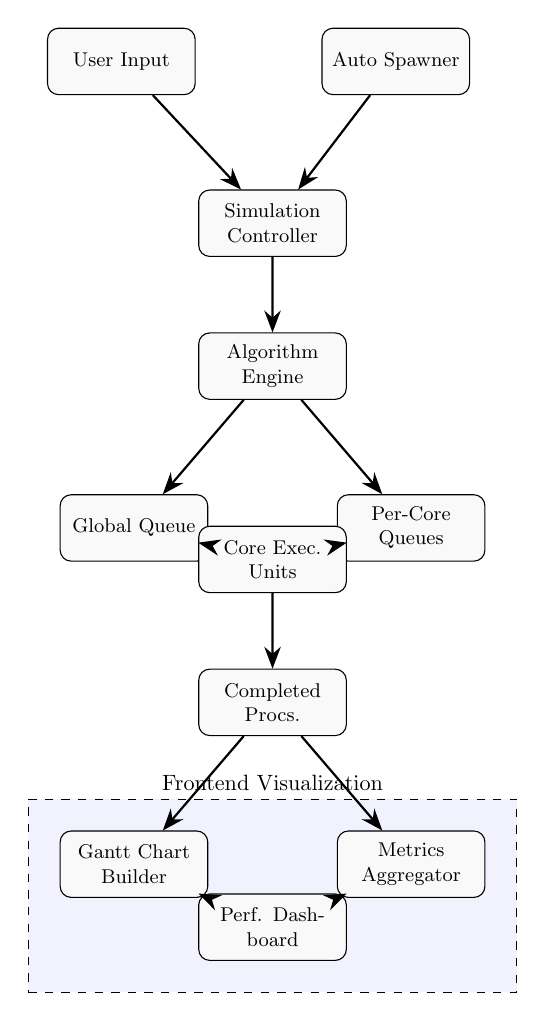
\begin{tikzpicture}[scale=0.8, transform shape, node distance=1.2cm, arrow/.style={-{Stealth[scale=1.2]}, thick}]
\tikzstyle{block} = [rectangle, draw, text width=6em, text centered, minimum height=3em, font=\small, fill=gray!5, rounded corners]
\node[block] (user) {User Input};
\node[block, right=2cm of user] (auto) {Auto Spawner};
\node[block, below=1.5cm of user, xshift=2.4cm] (sim) {Simulation Controller};
\draw[arrow] (user) -- (sim);
\draw[arrow] (auto) -- (sim);
\node[block, below=1.2cm of sim] (algo) {Algorithm Engine};
\draw[arrow] (sim) -- (algo);
\node[block, below=1.5cm of algo, xshift=-2.2cm] (global) {Global Queue};
\node[block, below=1.5cm of algo, xshift=2.2cm] (percore) {Per-Core Queues};
\draw[arrow] (algo) -- (global);
\draw[arrow] (algo) -- (percore);
\node[block, below=2cm of algo] (core) {Core Exec. Units};
\draw[arrow] (global) -- (core);
\draw[arrow] (percore) -- (core);
\node[block, below=1.2cm of core] (completed) {Completed Procs.};
\draw[arrow] (core) -- (completed);
\node[block, below=1.5cm of completed, xshift=-2.2cm] (gantt) {Gantt Chart Builder};
\node[block, below=1.5cm of completed, xshift=2.2cm] (metrics) {Metrics Aggregator};
\draw[arrow] (completed) -- (gantt);
\draw[arrow] (completed) -- (metrics);
\node[block, below=2.5cm of completed] (dashboard) {Perf. Dashboard};
\draw[arrow] (gantt) -- (dashboard);
\draw[arrow] (metrics) -- (dashboard);
\begin{scope}[on background layer]
\node[draw, dashed, fill=blue!5, inner sep=0.4cm, fit=(gantt) (metrics) (dashboard), label={Frontend Visualization}] {};
\end{scope}
\end{tikzpicture}
\caption{Logical System Flow and Module Organization}
\end{figure}

\section{Data Flow Diagrams}
The following analytical models visually decompose the system architecture into precise data flow operations and queues.

\subsection{Level 0: Context Diagram}
\begin{figure}[H]
\centering
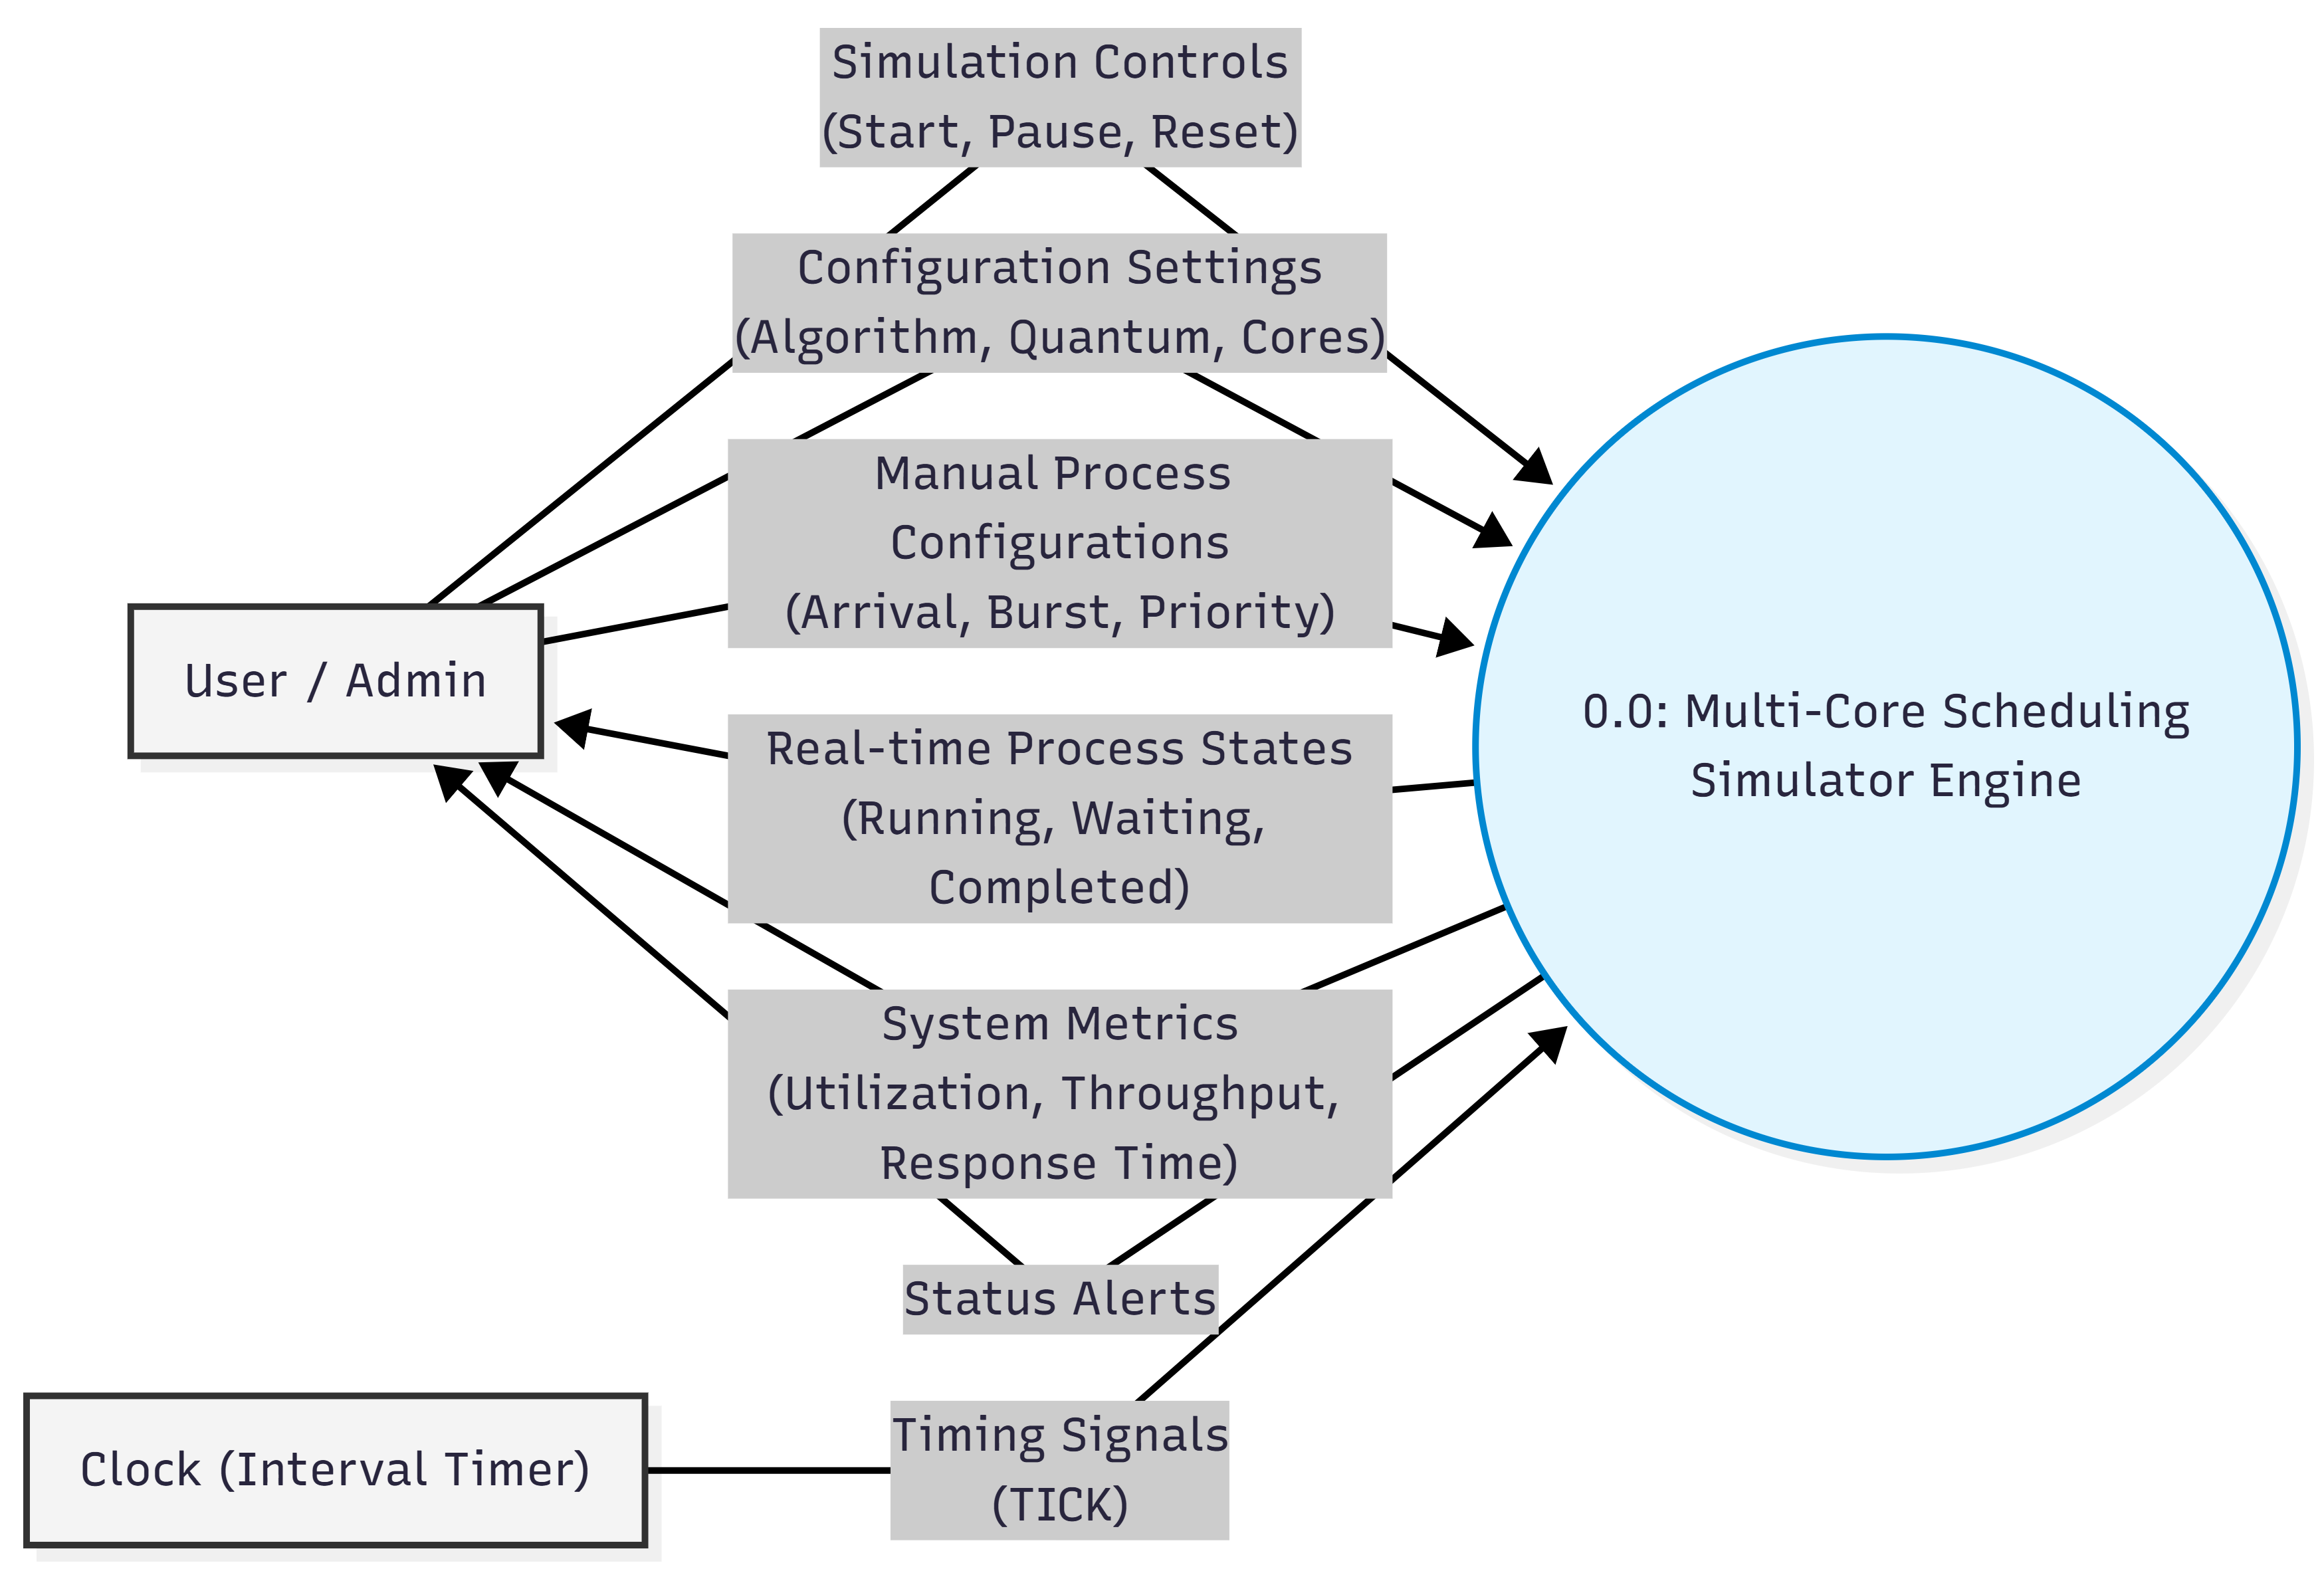
\includegraphics[width=0.8\textwidth]{Dfds/Multi-Core Scheduling-2026-04-21-151735.png}
\caption{Level 0 DFD: System Context Interactivity}
\end{figure}

\subsection{Level 1: Subsystem Architecture}
\begin{figure}[H]
\centering
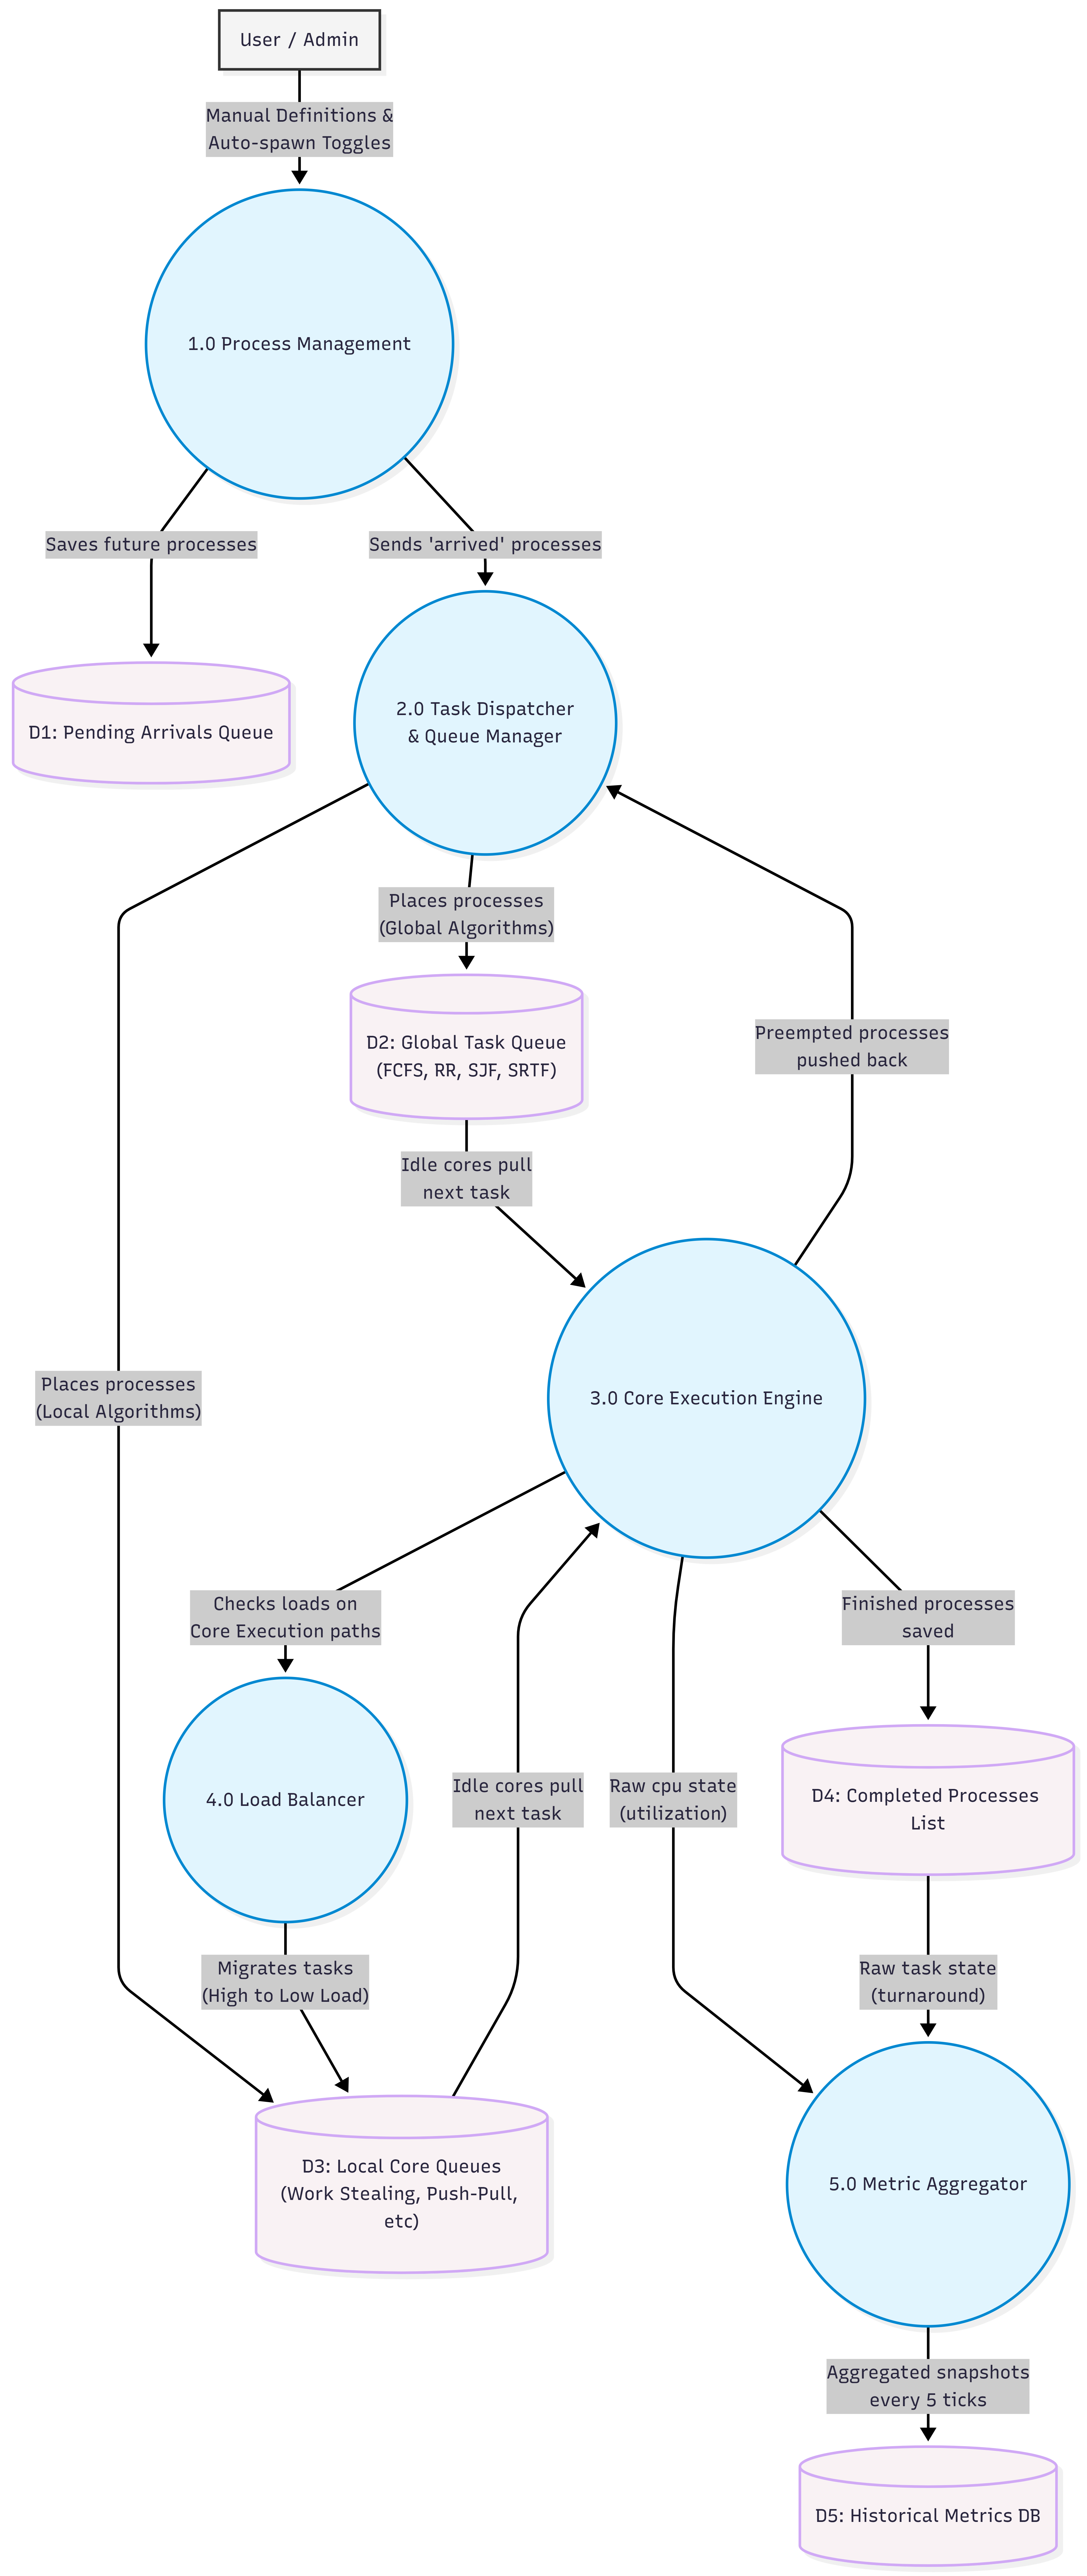
\includegraphics[width=0.95\textwidth]{Dfds/Multi-Core Scheduling-2026-04-21-151728.png}
\caption{Level 1 DFD: Major Functional Processes \& Data Queues}
\end{figure}

\subsection{Level 2: Deep Component Breakdowns}
\begin{figure}[H]
\centering
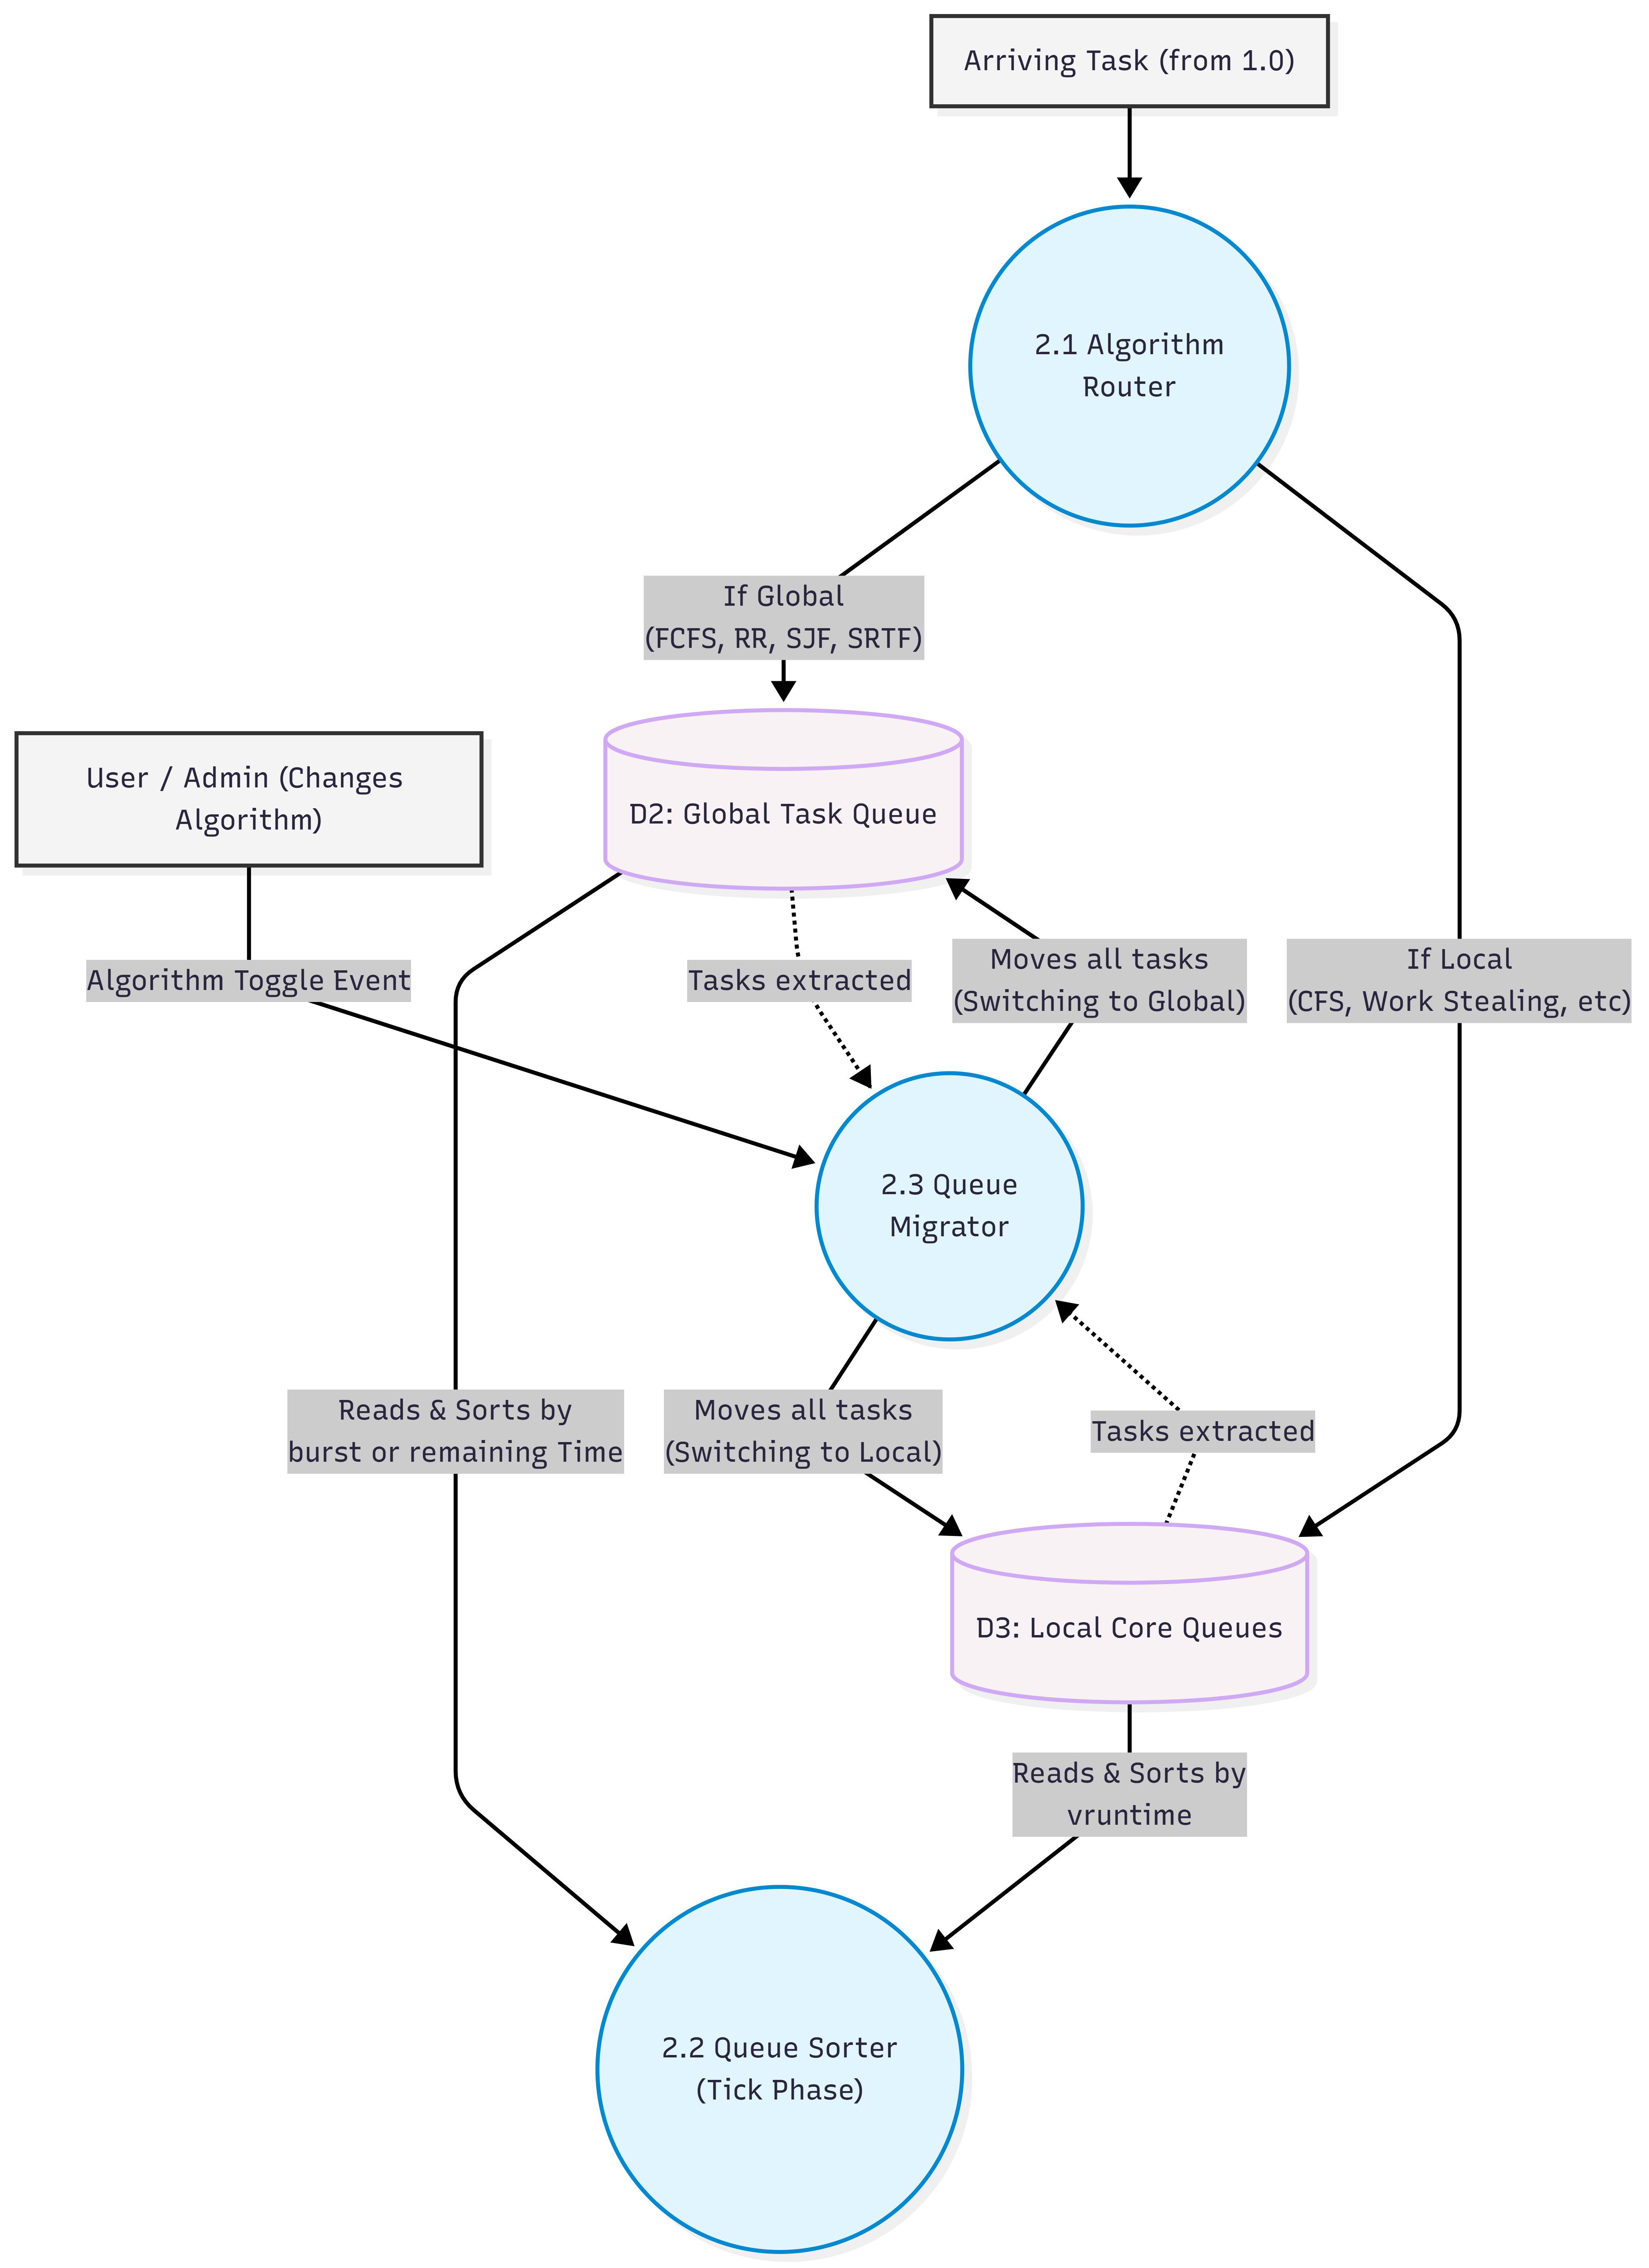
\includegraphics[width=0.85\textwidth]{Dfds/Multi-Core Scheduling-2026-04-21-151719.png}
\caption{Level 2.1 DFD: Task Dispatcher \& Queue Manager}
\end{figure}

\begin{figure}[H]
\centering
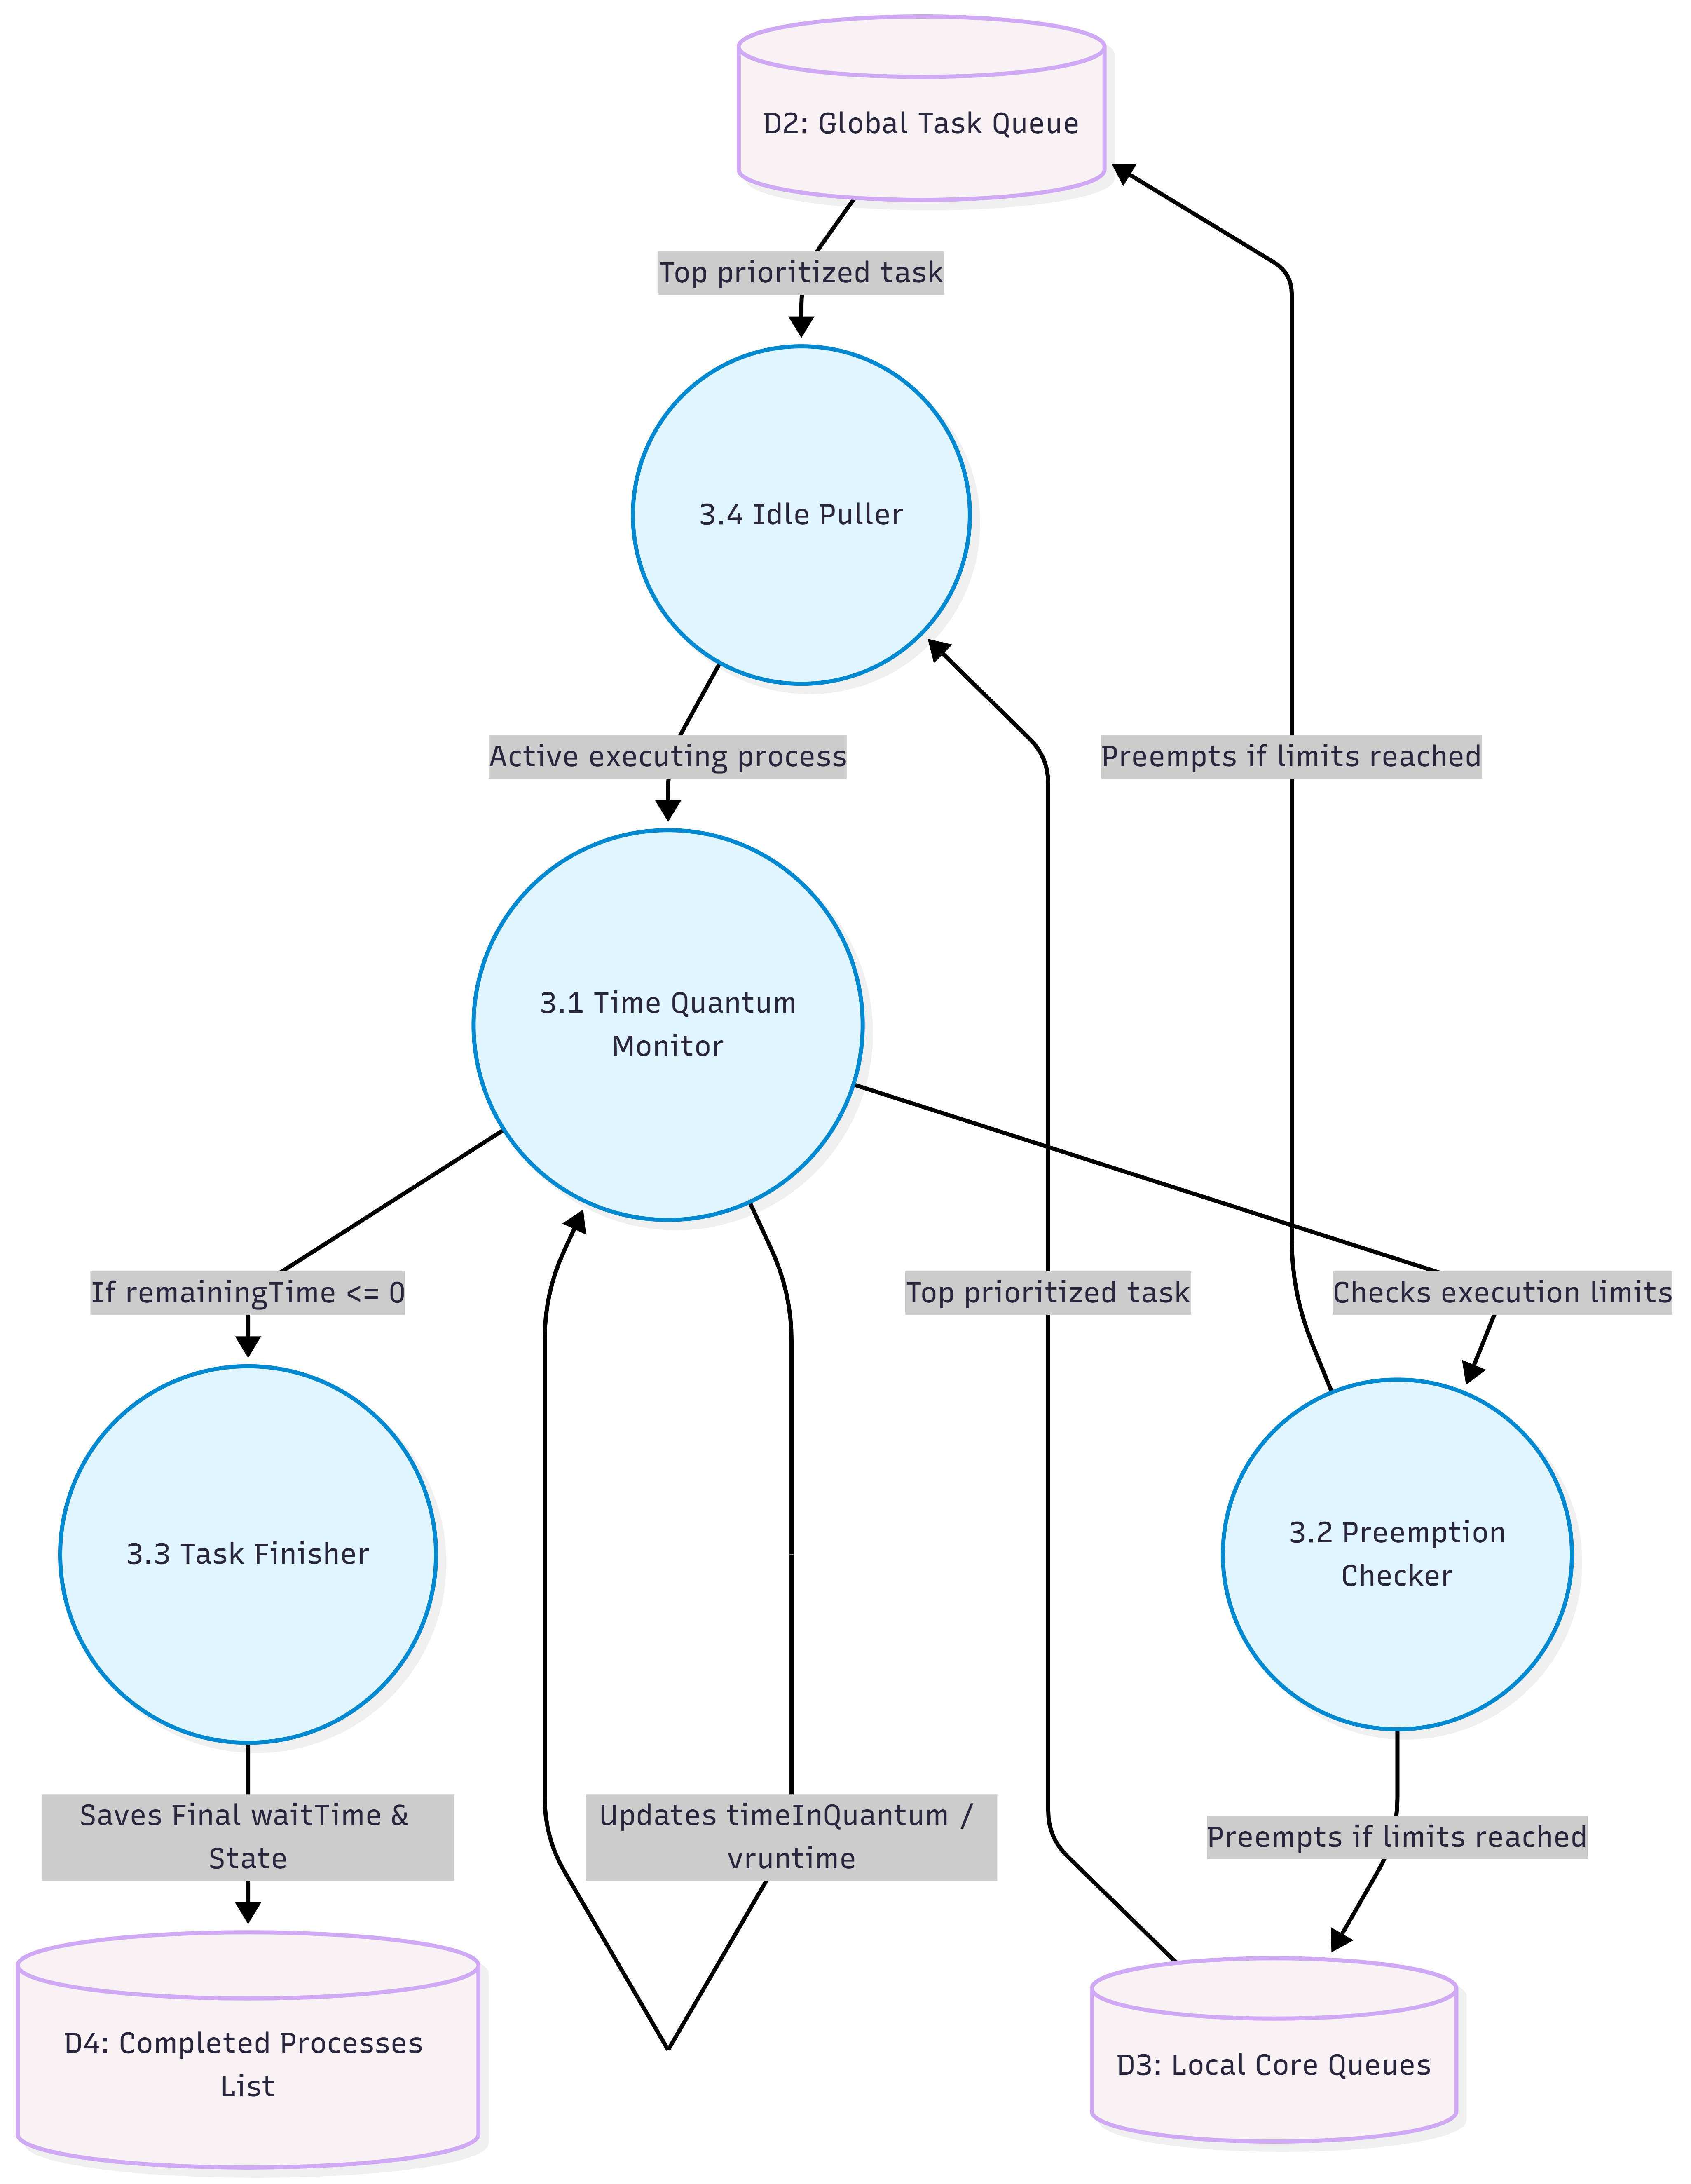
\includegraphics[width=0.85\textwidth]{Dfds/Multi-Core Scheduling-2026-04-21-151707.png}
\caption{Level 2.2 DFD: Core Execution Engine Lifecycle}
\end{figure}

\begin{figure}[H]
\centering
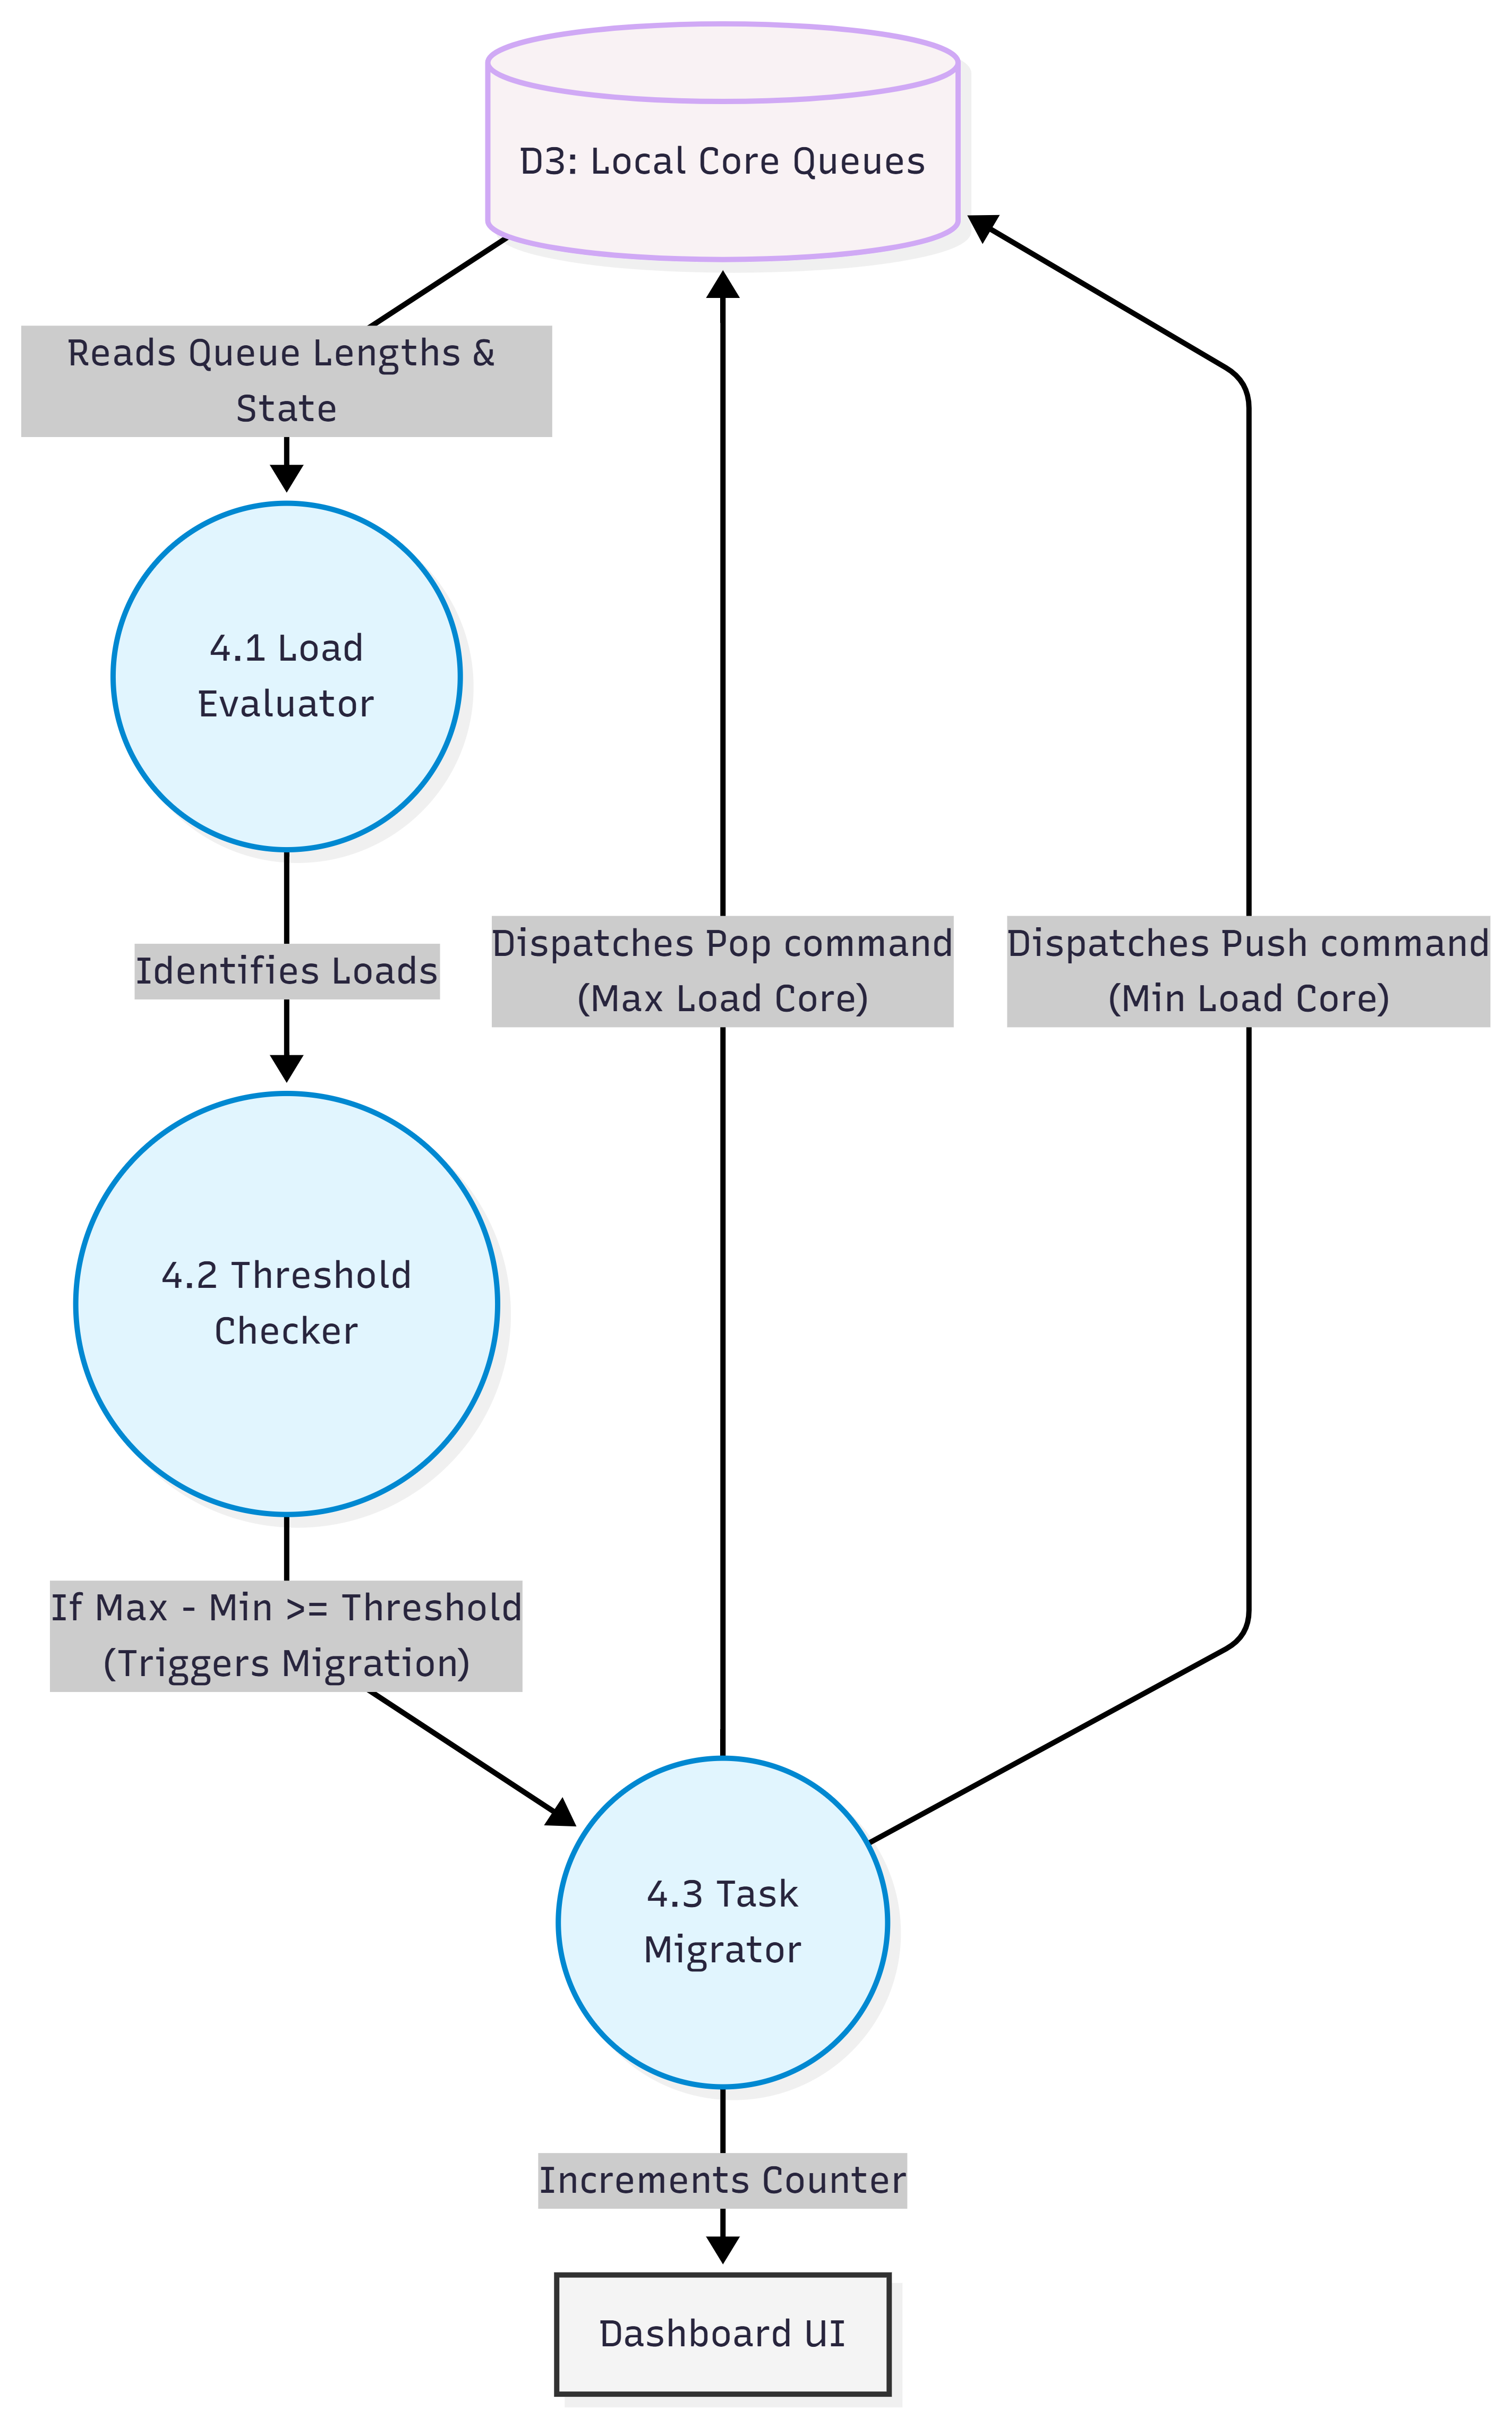
\includegraphics[width=0.85\textwidth]{Dfds/Multi-Core Scheduling-2026-04-21-151653.png}
\caption{Level 2.3 DFD: Dynamic Load Balancer}
\end{figure}

\begin{figure}[H]
\centering
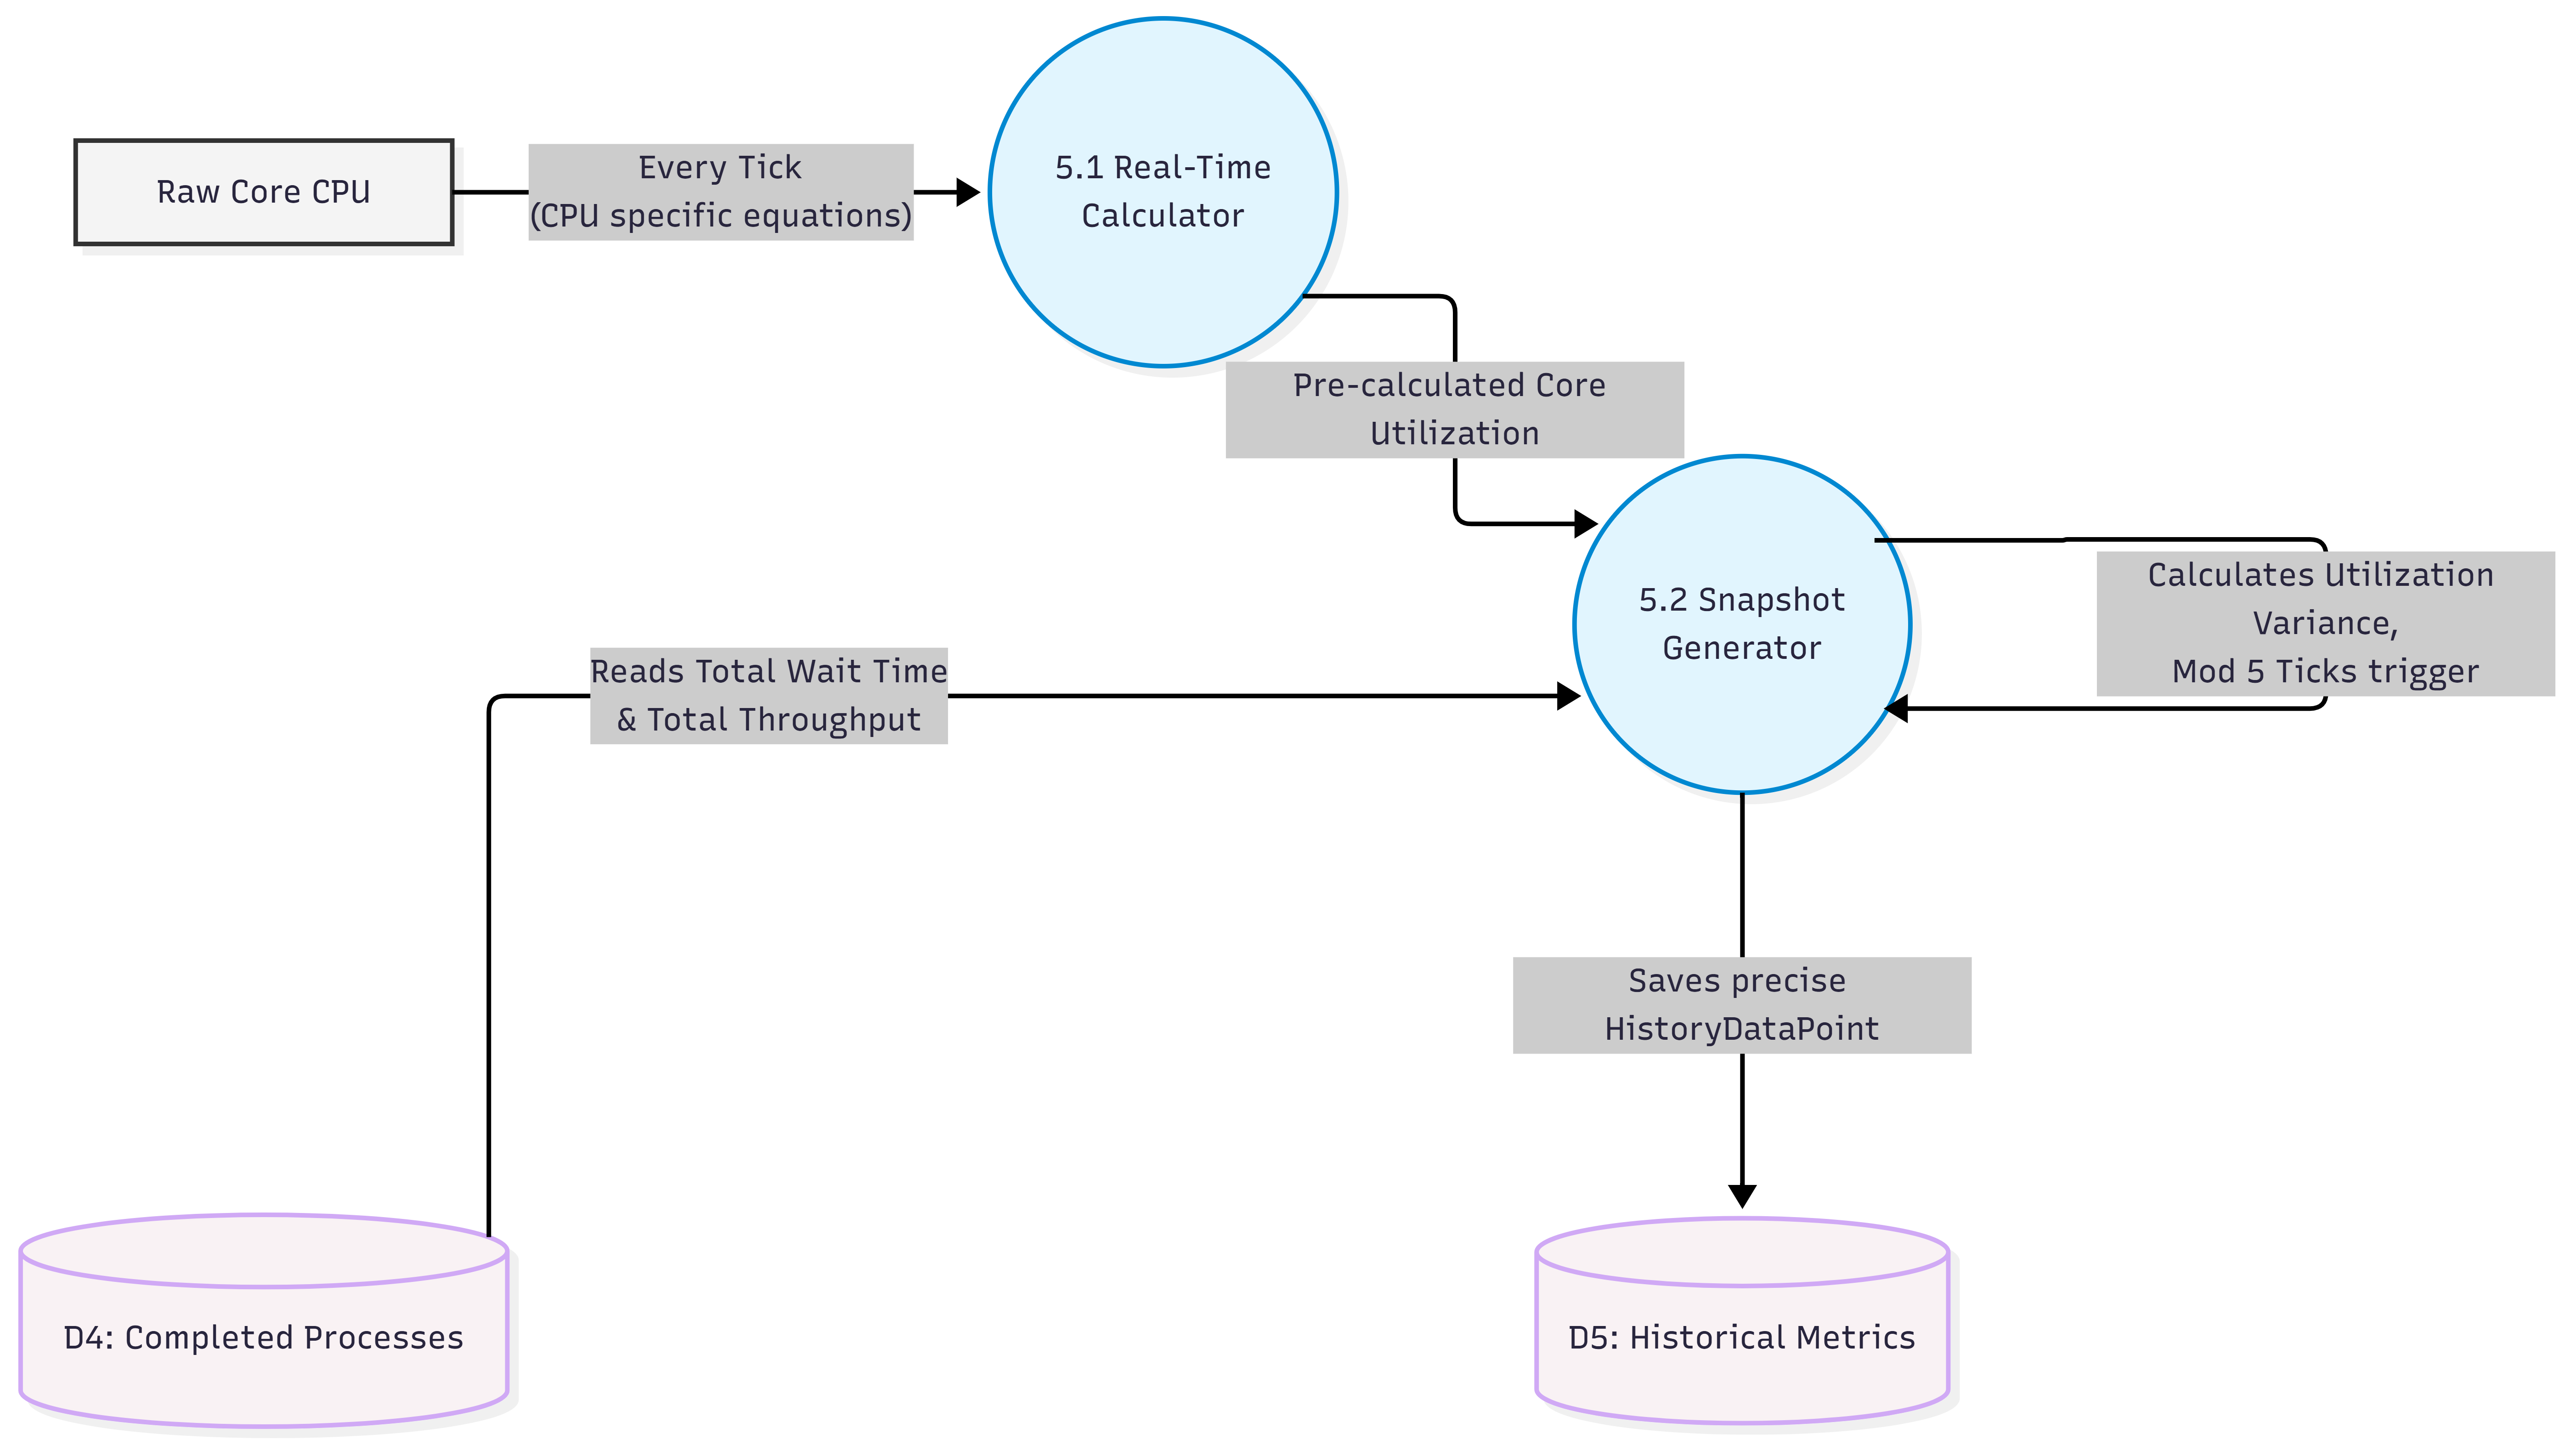
\includegraphics[width=0.85\textwidth]{Dfds/Multi-Core Scheduling-2026-04-21-151904.png}
\caption{Level 2.4 DFD: Real-Time Metrics Aggregator}
\end{figure}

\section{Revision Tracking on GitHub}
Continuous integration updates and active iteration history tracking can be found directly within the designated git repositories.
\\
\textbf{Repository Name:} Multi-Core-Load-Balancing-Scheduler\\
\textbf{GitHub Link:} \href{https://github.com/Syed-arsh-09/Multi-Core-Load-Balancing-Scheduler}{https://github.com/Syed-arsh-09/Multi-Core-Load-Balancing-Scheduler}

\section{Conclusion and Future Scope}
The Interactive Multi-Core CPU Scheduling Simulator successfully implements complex scheduling theories into an approachable, real-time environment. Through precise modeling mechanisms, the application functionally bridges statistical benchmarking execution against an elegant GUI interface.

\textbf{Future Scope:}
\begin{itemize}[noitemsep]
    \item Implementation of thread-level concurrency structures covering memory locks, read mechanisms, and strict mutexes implementations.
    \item Integration of network simulation protocols providing scope on expansive distributed systems alongside common isolated local threading arrays.
    \item Formatted extraction commands empowering users to export their analytical performance logs seamlessly as raw CSV documents for independent academic inspection.
\end{itemize}

\begin{thebibliography}{9}
\bibitem{silberschatz}
Abraham Silberschatz, Peter B. Galvin, and Greg Gagne,
\textit{Operating System Concepts}.

\bibitem{react}
React Documentation,
\url{https://react.dev/}.

\bibitem{recharts}
Recharts Data Visualization,
\url{https://recharts.org/}.
\end{thebibliography}


\appendix
\section{Appendix}

\subsection{AI-Generated Project Elaboration/Breakdown Report}

\textbf{1. Project Overview}\\
The objective of the "Interactive Multi-Core CPU Scheduling Simulator" is to build an educational data-visualization web application mapping Operating System process scheduling inside modern multi-core processors. The scope addresses multiple CPU scheduling algorithms (both single collective queues and distributed local queues) to let users observe system throughput, wait times, and core utilization in real-time. Expected outcomes include a functional sandbox where varied loads are tested against algorithms like Work Stealing, Shortest Job First, and Round Robin.

\textbf{2. Module-Wise Breakdown}
\begin{itemize}[noitemsep]
    \item \textbf{Simulation/State Module:} The mathematical core. It evaluates ticks based on designated algorithms, handles context switching, tracks total simulation time, and routes processes to available cores.
    \item \textbf{GUI Operations Module:} The visualization interface. It provides end-users the tools to dictate time quantums, inject manual procedures, toggle auto-spawning modes, and visually view each core's dedicated readiness queues.
    \item \textbf{Data Analytics Module:} The statistics center. Generates historical traces comparing metrics like CPU variance over time and relative throughput to provide verifiable comparisons.
\end{itemize}

\textbf{3. Functionalities}
\begin{itemize}[noitemsep]
    \item \textit{Simulation:} Tracks granular details like Time-In-Quantum, remaining burst times, and priority thresholds. Reallocates workload dynamically under the \texttt{PUSH\_PULL} strategy.
    \item \textit{GUI Operations:} Configurable parameters (ex: modifying multi-core scaling from 2 up to 16 cores), Gantt chart plotting with exact execution timestamps.
    \item \textit{Data Analytics:} Responsive line graphs that maintain history and allow hovering for exact point-in-time crosshair inspection.
\end{itemize}

\textbf{4. Technology Recommendations}
\begin{itemize}[noitemsep]
    \item \textbf{Languages:} JavaScript/TypeScript (ideal for web-based timeline environments), HTML/CSS.
    \item \textbf{Libraries:} React (Component decoupling), Tailwind CSS (Rapid styling), Recharts/Chart.js (Robust graph drawing), Framer Motion (Interpolated physics-based animations between DOM elements).
    \item \textbf{Tools:} Vite (Fast module bundling), Node.js, Git for collaborative tracking.
\end{itemize}

\textbf{5. Execution Plan}
\begin{itemize}[noitemsep]
    \item \textit{Step 1 (Foundations):} Setup Vite environment with React + TypeScript. Configure TailwindCSS directives. 
    \item \textit{Step 2 (The Engine):} Construct a central \texttt{useSimulation} React Hook capable of generating a standardized ticking loop (\texttt{setInterval}) and a standard \texttt{Process} interface definition.
    \item \textit{Step 3 (Algorithms):} Implement logic pathways starting with basic structures (FCFS, RR) and moving to heuristic models (CFS, Load Balancing).
    \item \textit{Step 4 (UI Building):} Map array outputs into distinct Core Visualizers, leveraging modern CSS to handle transition complexities.
    \item \textit{Step 5 (Analytics Integration):} Connect internal metric tallies to Recharts data models. Ensure UI bounds respect resize dimensions without overflow layout shifts.
    \item \textit{Step 6 (Polishing):} Inject tooltip interactions, responsive adjustments, and deploy to version control. Let the UI focus on dark modes or specific aesthetic themes for educational engagement.
\end{itemize}

\subsection{Problem Statement}
Modern task optimization fundamentally orbits operating systems structuring multi-core processor management. Operating system scheduling heavily influences system throughput yet traditional models remain strictly theoretical texts. An Interactive Platform transforms those ideas into tangible actions, thereby mitigating the lack of robust visual aids bridging practical processing mechanics together for active software educational validation.

\subsection{Solution / Core Engine Implementation}
The implementation spans multiple functional dimensions. Due to academic page constraints and modern decoupled web architecture, only the core algorithmic engine (\texttt{useSimulation.ts}) is attached below. This file represents the mathematical "brain" behind the scheduling algorithms, handling global queue states, active time quantums, and dynamic context tracking.

The expansive interactive graphical components (\texttt{Dashboard.tsx}), styling logic, and bundling configurations are omitted for brevity. However, the entire unabridged production repository can be fully evaluated via the GitHub reference securely listed within Section~6.

\vspace{1em}
\noindent\textbf{File snippet: \texttt{src/hooks/useSimulation.ts}}

\lstset{
  basicstyle=\ttfamily\scriptsize,
  keywordstyle=\color{blue}\bfseries,
  stringstyle=\color{red},
  commentstyle=\color{gray},
  numbers=left,
  numberstyle=\tiny\color{gray},
  stepnumber=1,
  breaklines=true,
  breakatwhitespace=false,
  showstringspaces=false,
  frame=lines,
  tabsize=2
}
\begin{lstlisting}
import { useEffect, useRef, useReducer, useCallback, useState } from 'react';
import type { Core, Process, SimulationMetrics, SchedulingAlgorithm, HistoryDataPoint } from '../types';

const TICK_RATE_MS = 50; 
const PROCESS_SPAWN_CHANCE = 0.05; // Lowered to 5% per tick to maintain stable system capacity (prevents queues from infinitely growing)

const generateId = () => Math.random().toString(36).substring(2, 6).toUpperCase();
const randomColor = () => {
  const colors = [
    '#ef4444', '#3b82f6', '#10b981', '#f59e0b', '#8b5cf6', '#ec4899', '#f97316'
  ];
  return colors[Math.floor(Math.random() * colors.length)];
};

const createInitialCores = (count = 4): Core[] => {
  return Array.from({ length: count }).map((_, i) => ({
    id: `core-${i}`,
    name: `Core ${i + 1}`,
    currentProcess: null,
    queue: [],
    utilization: 0,
    totalProcessedCount: 0,
  }));
};

const createProcess = (
  tickCount: number, 
  customProps?: { id?: string; burstTime?: number; arrivalTime?: number; priority?: number }
): Process => {
  const burst = customProps?.burstTime && customProps.burstTime > 0 ? customProps.burstTime : Math.floor(Math.random() * 40) + 20;
  return {
    id: customProps?.id || `P-${generateId()}`,
    arrivalTime: customProps?.arrivalTime !== undefined ? customProps.arrivalTime : tickCount,
    burstTime: burst,
    remainingTime: burst,
    priority: customProps?.priority !== undefined ? customProps.priority : 1,
    state: 'waiting',
    coreId: null,
    color: randomColor(),
    waitTime: 0,
    timeInQuantum: 0,
    vruntime: 0
  };
};

const assignProcessToCoreLocal = (process: Process, cores: Core[], algo: SchedulingAlgorithm) => {
  if (algo === 'AFFINITY') {
    // Deterministic modulo assignment simulating absolute CPU affinity based on strings
    let hash = 0;
    for (let i = 0; i < process.id.length; i++) hash += process.id.charCodeAt(i);
    const targetIdx = hash % cores.length;
    process.coreId = cores[targetIdx].id;
    cores[targetIdx].queue.push(process);
  } else {
    // Default fallback to least-loaded for Work Stealing / Push Pull / CFS
    let minLoad = Infinity;
    let targetCoreIdx = 0;
    cores.forEach((c, i) => {
      const load = c.queue.length + (c.currentProcess ? 1 : 0);
      if (load < minLoad) { minLoad = load; targetCoreIdx = i; }
    });
    process.coreId = cores[targetCoreIdx].id;
    cores[targetCoreIdx].queue.push(process);
  }
};

interface SimState {
  tickCount: number;
  cores: Core[];
  metrics: SimulationMetrics;
  completedProcesses: Process[];
  pendingArrivals: Process[]; 
  globalQueue: Process[];
  activeAlgorithm: SchedulingAlgorithm;
  timeQuantum: number;
  historicalMetrics: HistoryDataPoint[];
  migrationCounter: number;
}

const initialState: SimState = {
  tickCount: 0,
  cores: createInitialCores(4),
  metrics: { totalThroughput: 0, averageWaitTime: 0, tickCount: 0 },
  completedProcesses: [],
  pendingArrivals: [],
  globalQueue: [],
  activeAlgorithm: 'WORK_STEALING',
  timeQuantum: 15, // Default reasonable RR quantum
  historicalMetrics: [],
  migrationCounter: 0
};

type Action = 
  | { type: 'TICK'; autoSpawn: boolean }
  | { type: 'RESET'; coreCount: number }
  | { type: 'SET_ALGO'; algo: SchedulingAlgorithm }
  | { type: 'SET_TIME_QUANTUM'; quantum: number }
  | { type: 'SET_CORE_COUNT'; count: number }
  | { type: 'ADD_PROCESS'; id?: string; burstTime?: number; arrivalTime?: number; priority?: number };

function simReducer(state: SimState, action: Action): SimState {
  switch (action.type) {
    case 'RESET':
      return {
        ...initialState,
        activeAlgorithm: state.activeAlgorithm,
        timeQuantum: state.timeQuantum,
        cores: createInitialCores(action.coreCount),
        migrationCounter: 0
      };

    case 'SET_CORE_COUNT': {
      if (action.count === state.cores.length || action.count < 1) return state;
      const nextCores = state.cores.map(c => ({...c, queue: [...c.queue]}));
      const nextGlobal = [...state.globalQueue];

      if (action.count > state.cores.length) {
        const diff = action.count - state.cores.length;
        for (let i = 0; i < diff; i++) {
          nextCores.push({
            id: `core-${state.cores.length + i}`,
            name: `Core ${state.cores.length + i + 1}`,
            currentProcess: null,
            queue: [],
            utilization: 0,
            totalProcessedCount: 0
          });
        }
      } else {
        const removedCores = nextCores.splice(action.count);
        removedCores.forEach(c => {
          if (c.currentProcess) {
            c.currentProcess.coreId = null;
            c.currentProcess.state = 'waiting';
            nextGlobal.push(c.currentProcess);
          }
          c.queue.forEach(p => {
            p.coreId = null;
            nextGlobal.push(p);
          });
        });

        if (!['FCFS','RR','SJF','SRTF'].includes(state.activeAlgorithm)) {
          while(nextGlobal.length > 0) {
            let p = nextGlobal.shift()!;
            assignProcessToCoreLocal(p, nextCores, state.activeAlgorithm);
          }
        }
      }

      return {
        ...state,
        cores: nextCores,
        globalQueue: nextGlobal
      };
    }
    
    case 'SET_ALGO': {
      if (action.algo === state.activeAlgorithm) return state;

      const isGlobalTarget = ['FCFS','RR','SJF','SRTF'].includes(action.algo);
      const wasGlobal = ['FCFS','RR','SJF','SRTF'].includes(state.activeAlgorithm);
      let nextGlobal = [...state.globalQueue];
      let nextCores = state.cores.map(c => ({...c, queue: [...c.queue]}));

      // Queue State Migration
      if (isGlobalTarget && !wasGlobal) {
        // Collect all local queues into global queue
        nextCores.forEach(c => {
          while (c.queue.length > 0) {
            let p = c.queue.shift()!;
            p.coreId = null;
            nextGlobal.push(p);
          }
        });
      } else if (!isGlobalTarget && wasGlobal) {
        // Scatter global queue into local queues
        while (nextGlobal.length > 0) {
          let p = nextGlobal.shift()!;
          assignProcessToCoreLocal(p, nextCores, action.algo);
        }
      } else if (!isGlobalTarget && !wasGlobal && action.algo === 'AFFINITY') {
         // Migrating from local to local with Affinity
         // Re-hash everything
         let allProcs: Process[] = [];
         nextCores.forEach(c => {
            while (c.queue.length > 0) allProcs.push(c.queue.shift()!);
         });
         allProcs.forEach(p => assignProcessToCoreLocal(p, nextCores, action.algo));
      }

      // Bridge the chart gap: record a metric snapshot for the NEW algorithm
      // at the current tick so there's no X-axis discontinuity on the graph.
      const bridgeHistory = [...state.historicalMetrics];
      const avgUtil = nextCores.reduce((s, c) => s + c.utilization, 0) / nextCores.length;
      const utilVar = nextCores.reduce((s, c) => s + Math.pow(c.utilization - avgUtil, 2), 0) / nextCores.length;
      const completedAll = state.completedProcesses;
      const avgResp = completedAll.length > 0
        ? completedAll.reduce((s, p) => s + p.waitTime + p.burstTime, 0) / completedAll.length
        : 0;
      const elapsed = (state.tickCount * 50) / 1000; // TICK_RATE_MS = 50
      const tpRate = elapsed > 0 ? Math.round((state.metrics.totalThroughput / elapsed) * 100) / 100 : 0;
      bridgeHistory.push({
        tick: state.tickCount,
        algorithm: action.algo,
        avgWaitTime: state.metrics.averageWaitTime,
        throughput: tpRate,
        utilization: avgUtil,
        utilizationVariance: Math.round(utilVar * 100) / 100,
        responseTime: Math.round(avgResp * 10) / 10,
        migrationCount: state.migrationCounter
      });

      return {
        ...state,
        activeAlgorithm: action.algo,
        globalQueue: nextGlobal,
        cores: nextCores,
        historicalMetrics: bridgeHistory
      };
    }
    
    case 'SET_TIME_QUANTUM': {
      return { ...state, timeQuantum: Math.max(1, action.quantum) };
    }

    case 'ADD_PROCESS': {
      const newProcess = createProcess(state.tickCount, {
        id: action.id,
        burstTime: action.burstTime,
        arrivalTime: action.arrivalTime,
        priority: action.priority
      });
      
      if (newProcess.arrivalTime > state.tickCount) {
        return {
          ...state,
          pendingArrivals: [...state.pendingArrivals, newProcess].sort((a, b) => a.arrivalTime - b.arrivalTime)
        };
      } 

      const nextGlobal = [...state.globalQueue];
      const nextCores = [...state.cores.map(c => ({...c, queue: [...c.queue]}))];
      
      if (['FCFS','RR','SJF','SRTF'].includes(state.activeAlgorithm)) {
        nextGlobal.push(newProcess);
      } else {
        assignProcessToCoreLocal(newProcess, nextCores, state.activeAlgorithm);
      }
      
      return { ...state, cores: nextCores, globalQueue: nextGlobal };
    }

    case 'TICK': {
      let nextTick = state.tickCount + 1;
      let nextCores = state.cores.map(c => ({ ...c, queue: [...c.queue] }));
      let nextGlobal = [...state.globalQueue.map(p => ({ ...p, waitTime: p.waitTime + 1}))];
      let nextCompleted = [...state.completedProcesses];
      let nextPending = [...state.pendingArrivals];
      let nextHistory = [...state.historicalMetrics];
      let nextMetrics = { 
        ...state.metrics, 
        tickCount: nextTick 
      };

      // 0. Dispatch processes that officially arrived this tick
      const readyToDispatch = nextPending.filter(p => p.arrivalTime <= nextTick);
      nextPending = nextPending.filter(p => p.arrivalTime > nextTick);
      
      readyToDispatch.forEach(p => {
        if (['FCFS','RR','SJF','SRTF'].includes(state.activeAlgorithm)) {
          nextGlobal.push(p);
        } else {
          assignProcessToCoreLocal(p, nextCores, state.activeAlgorithm);
        }
      });

      // 1. Process Generation (Auto Spawn)
      if (action.autoSpawn && Math.random() < PROCESS_SPAWN_CHANCE) {
        const newProcess = createProcess(nextTick);
        if (['FCFS','RR','SJF','SRTF'].includes(state.activeAlgorithm)) {
          nextGlobal.push(newProcess);
        } else {
          assignProcessToCoreLocal(newProcess, nextCores, state.activeAlgorithm);
        }
      }

      // 2. Sorting Phase based on Algorithm
      if (state.activeAlgorithm === 'FCFS' || state.activeAlgorithm === 'RR') {
        // FCFS and RR use simple arrival time queue behavior, do nothing (Queue naturally maintains order)
      } else if (state.activeAlgorithm === 'SJF') {
        nextGlobal.sort((a, b) => a.burstTime - b.burstTime); 
      } else if (state.activeAlgorithm === 'SRTF') {
        nextGlobal.sort((a, b) => a.remainingTime - b.remainingTime);
      } else if (state.activeAlgorithm === 'CFS') {
        nextCores.forEach(c => c.queue.sort((a, b) => a.vruntime - b.vruntime));
      }

      // 3. Execution Phase
      nextCores = nextCores.map(core => {
        let c = { ...core };
        
        // Update waiting times inside local queues
        c.queue = c.queue.map(p => ({ 
          ...p, 
          waitTime: p.waitTime + 1,
          vruntime: state.activeAlgorithm === 'CFS' ? p.vruntime - (p.priority * 0.05) : p.vruntime
        }));

        if (c.currentProcess) {
          let p = { ...c.currentProcess };
          p.remainingTime -= 1;
          p.timeInQuantum += 1;
          if (state.activeAlgorithm === 'CFS') p.vruntime += 1;
          
          if (p.remainingTime <= 0) {
            // Process Finished
            p.state = 'completed';
            nextCompleted.push(p);
            if (nextCompleted.length > 50) nextCompleted.shift(); // Keep last 50
            
            nextMetrics.totalThroughput += 1;
            nextMetrics.averageWaitTime = 
              ((nextMetrics.averageWaitTime * (nextMetrics.totalThroughput - 1)) + p.waitTime) 
              / nextMetrics.totalThroughput;
            
            c.totalProcessedCount += 1;
            c.currentProcess = null;
          } else {
             // Preemption Checking
             let preempt = false;
             if (state.activeAlgorithm === 'RR' && p.timeInQuantum >= state.timeQuantum) {
               preempt = true;
             } else if (state.activeAlgorithm === 'SRTF' && nextGlobal.length > 0 && nextGlobal[0].remainingTime < p.remainingTime) {
               preempt = true;
             } else if (state.activeAlgorithm === 'CFS' && c.queue.length > 0 && c.queue[0].vruntime < p.vruntime - 5) { // vruntime delta of 5
               preempt = true;
             }

             if (preempt) {
               p.state = 'waiting';
               p.timeInQuantum = 0;
               if (['RR','SRTF'].includes(state.activeAlgorithm)) {
                 p.coreId = null;
                 nextGlobal.push(p);
               } else {
                 c.queue.push(p); // Re-queues local
               }
               c.currentProcess = null;
             } else {
               c.currentProcess = p; // Continue running
             }
          }
        }

        // 4. Fill Idle Cores
        if (!c.currentProcess) {
          if (['FCFS','RR','SJF','SRTF'].includes(state.activeAlgorithm)) {
            if (nextGlobal.length > 0) {
              c.currentProcess = nextGlobal.shift()!;
              c.currentProcess.coreId = c.id;
              c.currentProcess.state = 'running';
            }
          } else {
            if (c.queue.length > 0) {
              c.currentProcess = c.queue.shift()!;
              c.currentProcess.state = 'running';
            }
          }
        }
        
        const isBusy = c.currentProcess ? 100 : 0;
        c.utilization = (c.utilization * 0.95) + (isBusy * 0.05);

        return c;
      });

      // 5. Load balancing patterns (WORK_STEALING & PUSH_PULL)
      let tickMigrations = 0;
      if (state.activeAlgorithm === 'WORK_STEALING' || state.activeAlgorithm === 'PUSH_PULL') {
        const loads = nextCores.map(c => c.queue.length + (c.currentProcess ? 1 : 0));
        let maxLoadIdx = loads.indexOf(Math.max(...loads));
        let minLoadIdx = loads.indexOf(Math.min(...loads));
        
        const threshold = state.activeAlgorithm === 'PUSH_PULL' ? 1 : 2; 
        
        if (loads[maxLoadIdx] - loads[minLoadIdx] >= threshold && nextCores[maxLoadIdx].queue.length > 0) {
           const stolen = nextCores[maxLoadIdx].queue.pop();
           if (stolen) {
             stolen.coreId = nextCores[minLoadIdx].id;
             nextCores[minLoadIdx].queue.push(stolen);
             tickMigrations += 1;
           }
        }
      }

      // 6. Snapshots for Analytics Engine
      const nextMigrationCounter = state.migrationCounter + tickMigrations;
      if (nextTick % 5 === 0) {
        const avgUtilization = nextCores.reduce((s,c) => s + c.utilization, 0) / nextCores.length;
        // CPU Utilization Variance
        const utilVariance = nextCores.reduce((s,c) => s + Math.pow(c.utilization - avgUtilization, 2), 0) / nextCores.length;
        // Response Time (avg turnaround = avgWaitTime + avgBurstTime of completed)
        const completedAll = nextCompleted;
        const avgResponseTime = completedAll.length > 0
          ? completedAll.reduce((s, p) => s + p.waitTime + p.burstTime, 0) / completedAll.length
          : 0;
        // Throughput rate (jobs per second)
        const elapsedSeconds = (nextTick * TICK_RATE_MS) / 1000;
        const throughputRate = elapsedSeconds > 0 ? Math.round((nextMetrics.totalThroughput / elapsedSeconds) * 100) / 100 : 0;

        nextHistory.push({
          tick: nextTick,
          algorithm: state.activeAlgorithm,
          avgWaitTime: nextMetrics.averageWaitTime,
          throughput: throughputRate,
          utilization: avgUtilization,
          utilizationVariance: Math.round(utilVariance * 100) / 100,
          responseTime: Math.round(avgResponseTime * 10) / 10,
          migrationCount: nextMigrationCounter
        });
        if (nextHistory.length > 600) nextHistory.shift(); // Keep last 600 data points
      }

      return {
        tickCount: nextTick,
        cores: nextCores,
        globalQueue: nextGlobal,
        completedProcesses: nextCompleted,
        pendingArrivals: nextPending,
        historicalMetrics: nextHistory,
        metrics: nextMetrics,
        activeAlgorithm: state.activeAlgorithm,
        timeQuantum: state.timeQuantum,
        migrationCounter: nextMigrationCounter
      };
    }
    default:
      return state;
  }
}

export function useSimulation() {
  const [isRunning, setIsRunning] = useState(false);
  const [isAutoSpawn, setIsAutoSpawn] = useState(false); 
  
  const [state, dispatch] = useReducer(simReducer, initialState);
  const intervalRef = useRef<number | null>(null);

  const tick = useCallback(() => {
    dispatch({ type: 'TICK', autoSpawn: isAutoSpawn });
  }, [isAutoSpawn]);

  useEffect(() => {
    if (isRunning) {
      intervalRef.current = window.setInterval(tick, TICK_RATE_MS);
    } else if (intervalRef.current) {
      window.clearInterval(intervalRef.current);
    }
    return () => {
      if (intervalRef.current) window.clearInterval(intervalRef.current);
    };
  }, [isRunning, tick]);

  useEffect(() => {
    if (isRunning && !isAutoSpawn && state.tickCount > 0) {
      const isIdle = state.cores.every(c => c.queue.length === 0 && !c.currentProcess);
      const isPendingEmpty = state.pendingArrivals.length === 0;
      const isGlobalEmpty = state.globalQueue.length === 0;
      if (isIdle && isPendingEmpty && isGlobalEmpty) {
        setIsRunning(false);
      }
    }
  }, [state.cores, state.pendingArrivals, state.globalQueue, isRunning, isAutoSpawn, state.tickCount]);

  const toggleSimulation = () => setIsRunning(!isRunning);
  const toggleAutoSpawn = () => setIsAutoSpawn(!isAutoSpawn);
  const setAlgorithm = (algo: SchedulingAlgorithm) => dispatch({ type: 'SET_ALGO', algo });
  const setTimeQuantum = (quantum: number) => dispatch({ type: 'SET_TIME_QUANTUM', quantum });
  const setCoreCount = (count: number) => dispatch({ type: 'SET_CORE_COUNT', count });
  
  const addProcess = (params?: { id?: string; burstTime?: number; arrivalTime?: number; priority?: number }) => {
    dispatch({ type: 'ADD_PROCESS', ...params });
  };

  const reset = () => {
    setIsRunning(false);
    dispatch({ type: 'RESET', coreCount: state.cores.length });
    setIsAutoSpawn(false);
  };

  return {
    ...state,
    isRunning,
    isAutoSpawn,
    toggleSimulation,
    toggleAutoSpawn,
    setAlgorithm,
    setTimeQuantum,
    setCoreCount,
    addProcess,
    reset,
  };
}
\end{lstlisting}

\end{document}
